

\begin{enumerate}
	\item{
	%Part a
	The circuit is converted to the s domain:
	\begin{figure}[H]
		\centering
		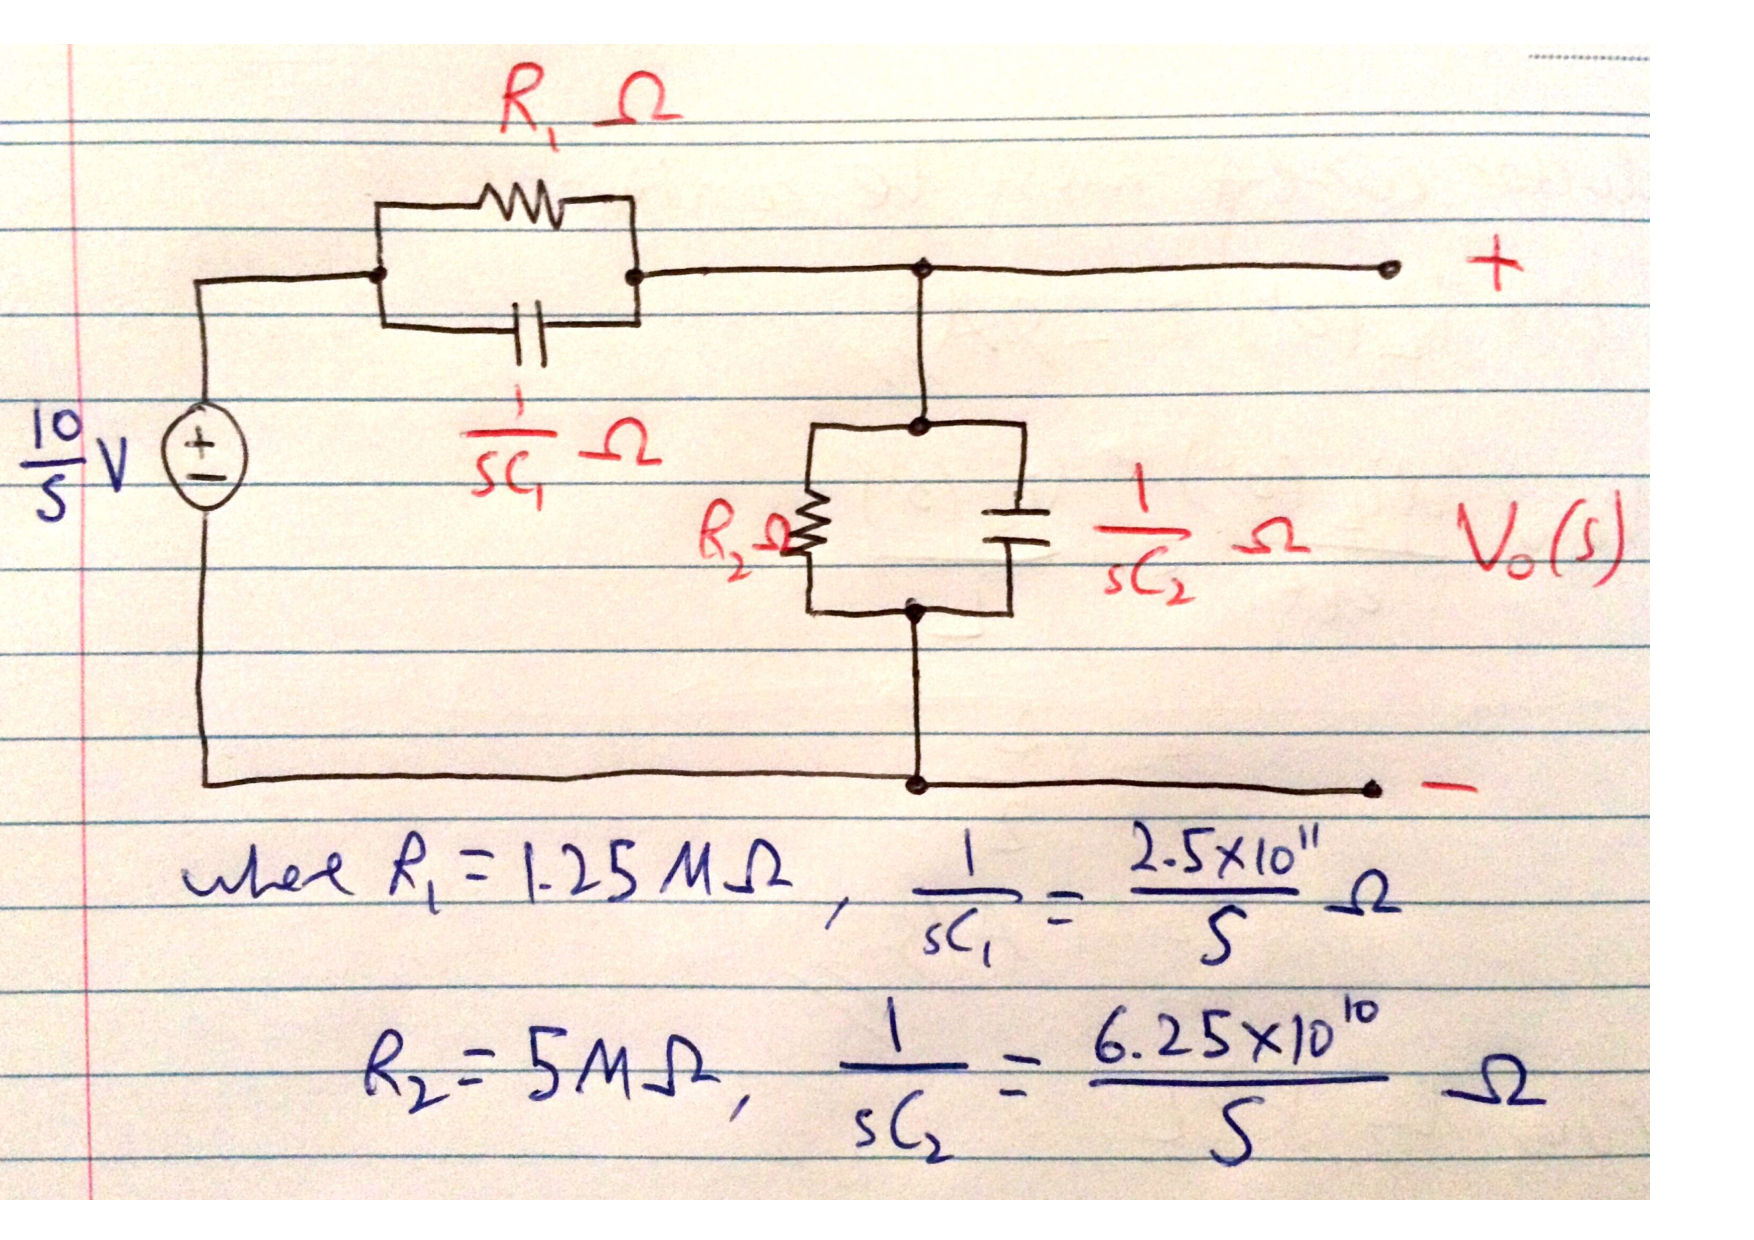
\includegraphics[scale=0.54]{q1a.pdf}
	\end{figure}
	}

	\item{
	%Part b
		\begin{align*}
			Z_{eq1} &= \left( \frac{1}{Z_{R_1}} +								%NEXTLINE
			\frac{1}{Z_{C_1}} \right)^{-1} \\
			&= \left(\frac{1}{1.25 \times 10^6} + 								%NEXTLINE
			s \cdot 4 \times 10^{-12}\right)^{-1} \\
			&= \left(\frac{1 + 1.25\times 10^6 \cdot (s \cdot 4 \times 10^{-12})%NEXTLINE
			}{ 1.25\times 10^6} \right)^{-1} \\
			&= \frac{1.25\times 10^6}{1 + 1.25\times 10^6 						%NEXTLINE
			\cdot (s \cdot 4 \times 10^{-12})} \\ 
			\\
			\therefore Z_{eq1} &= \frac{2.5 \times 10^{11}}{s + 2 \times 10^5} \ \Omega
		\end{align*}
	}

	\item{
	%Part c
		\begin{align*}
			Z_{eq2} &= \left( \frac{1}{Z_{R_2}} +								%NEXTLINE
			\frac{1}{Z_{C_2}} \right)^{-1} \\
			&= \left( \frac{1}{5\times 10^6} +									%NEXTLINE
			s \cdot 16 \times 10^{-12} \right)^{-1} \\
			&= \left( \frac{1 + 5\times 10^6 \cdot								%NEXTLINE
			(s \cdot 16 \times 10^{-12})}{5\times 10^6} \right)^{-1} \\
			&= \frac{5 \times 10^6}{1 + 5\times 10^6 							%NEXTLINE
			\cdot(s \cdot 16 \times 10^{-12})} \\
			\\
			\therefore Z_{eq2} &= \frac{6.25 \times 10^{10}}{s + 1.25 \times 10^4} \ \Omega
		\end{align*}
		\\
	}

	\item{
	%Part d
		Using voltage division:
		\begin{align*}
			V_o(s) &= V_{in}(s) \cdot \frac{Z_{eq2}}{Z_{eq1} + Z_{eq2}}\\
			&= \frac{10}{s} \cdot \frac{\dfrac{6.25 \times 10^{10}}				%NEXTLINE
			{s + 1.25 \times 10^4}}{\dfrac{6.25 \times 10^{10}}					%NEXTLINE
			{s + 1.25 \times 10^4} + \dfrac{2.5 \times 10^{11}}					%NEXTLINE
			{s + 2 \times 10^5}} \\
			&= \frac{10}{s} \cdot \frac{\dfrac{6.25 \times 10^{10}}             %NEXTLINE
			{s+1.25 \times 10^4}}{\dfrac{(6.25 \times 10^{10})					%NEXTLINE
			(s + 2\times 10^5) + (2.5 \times 10^{11})(s + 1.25 \times 10^4)}	%NEXTLINE
			{(s + 1.25 \times 10^4)\cdot(s + 2 \times 10^5)}} \\
			&= \frac{10}{s} \cdot \frac{6.25 \times 10^{10}}            
			{s+1.25 \times 10^4} \cdot \frac{(s + 1.25 \times 10^4)
			\cdot(s + 2 \times 10^5)}{(6.25 \times 10^{10})
			(s + 2\times 10^5) + (2.5 \times 10^{11})
			(s + 1.25 \times 10^4)} \\
			&= \frac{6.25 \times 10^{11} \cdot (s + 1.25 \times 10^4) \cdot 
			(s + 2 \times 10^5)}{3.125 \times 10^{11} \cdot s \cdot 
			(s + 1.25 \times 10^4) \cdot (s + 5 \times 10^4)} \\
			&= \frac{2 \cdot (s + 2 \times 10^5)}
			{s \cdot (s + 5 \times 10^4)} \\ 
			\\
			\therefore V_o(s) &= \frac{2s + 4 \times 10^5}{s^2 + 5 \times 10^4 \cdot s} \ \mathrm{V} \\
		\end{align*}
		Now perform partial fraction expansion:
		\begin{align*}
			\frac{2s + 4 \times 10^5}{s^2 + 5 \times 10^4 \cdot s} &= 
			\frac{A}{s} + \frac{B}{s + 50000} \\
			A(s+50000) + Bs &= 2(s + 200000) \\
			(s = 0): \; 50000A &= 400000 \\
			\implies A &= 8 \\
			(s = -50000): \;  -50000B &= 300000 \\
			\implies B &= -6 \\
		\end{align*}
		\begin{equation*}
			\therefore V_o(s) = \frac{8}{s} - \frac{6}{s + 50000} \ \mathrm{V}
		\end{equation*}
		\\
		Perform inverse Laplace transform to find $v_o(t)$:
		\begin{align*}
			v_o(t) &= \mathcal{L}^{-1} [V_o(s)]\\
			&= \mathcal{L}^{-1} \left[\frac{8}{s} - \frac{6}{s + 50000}\right] \\
			\\
			\therefore v_o(t) &= \left(8 -6 e^{-50000t} \right) u(t) \ \mathrm{V}
		\end{align*}
		\\
	}

	\item{
	%Part e
		Using Ohm's Law in s domain:
		\begin{align*}
			V_{in}(s) &= Z_{eq} I_o(s) \\
			&= (Z_{eq1} + Z_{eq2}) I_o(s) \\
			\\
			\therefore I_o(s) &= \frac{V_{in}(s)}{Z_{eq1} + Z_{eq2}} \\
			&= \frac{\dfrac{10}{s}} 
			{\dfrac{2.5 \times 10^{11}}
			{s + 2 \times 10^5} + \dfrac{6.25 \times 10^{10}}{s + 1.25 \times 10^4}} \\
			&= \frac{\dfrac{10}{s}} 
			{\dfrac{3.125 \times 10^{11} (s + 50000)}{(s+12500)(s+200000)}} \\
			&= \frac{(s+12500)(s+200000)}{3.125 \times 10^{10} s (s + 50000)} \ \mathrm{A} \\
		\end{align*}
		We note that the order of the numberator polynomial is equal to the order of the denominator polynomial, and so to perform partial fraction expansion we must first perform polynomial division:
		\\
		\begin{equation*}
			\frac{(s+12500)(s+200000)}{3.125 \times 10^{10} s (s + 50000)} = 3.2\times10^{-11} + \frac{5.2\times10^{-6}s + 8\times10^{-2}}{s(s+5\times10^4)}
		\end{equation*}
		\\
		Now perform partial fraction expansion:
		\begin{align*}
			\frac{5.2\times10^{-6}s + 8\times10^{-2}}{s(s+5\times10^4)} &= \frac{A}{s} + \frac{B}{s+5\times10^4} \\
			\therefore 5.2\times10^{-6}s + 8\times10^{-2} &= A(s+5\times10^4) + Bs \\
		\end{align*}
		\begin{equation*}
			s = 0 \implies 8\times10^{-2} = A(5\times10^4) \implies A = 1.6\times10^{-6}
		\end{equation*}
		\begin{equation*}
			s = -5\times10^4 \implies -0.18 = B(-5\times10^4) \implies B = 3.6\times10^{-6} \\
		\end{equation*}
		\\
		Now the current in the s domain can be represented in partial fraction expanded form:
		\begin{align*}
			I_o(s) &= 3.2\times10^{-11} + \frac{1.6\times10^{-6}}{s} + \frac{3.6\times10^{-6}}{s+5\times10^4} \ \mathrm{A} \\
			&= 3.2\times10^{-5} + \frac{1.6}{s} + \frac{3.6}{s+5\times10^4} \ \mu \mathrm{A}
		\end{align*}
		Using inverse Laplace transform to find $i_o(t)$.
		\begin{align*}
			i_o(t) &= \mathcal{L}^{-1}\left[ I_o(s) \right] \\
			&= \mathcal{L}^{-1} \left[3.2\times10^{-5} + \frac{1.6}{s} + \frac{3.6}{s+5\times10^4} \right] \\
			\\
			\therefore i_o(t) &= 3.2 \times 10^{-5} \cdot \delta(t) + \left(1.6 + 3.6 \times e^{-50000t} \right) u(t) \ \mu \mathrm{A}
		\end{align*}
	}

\end{enumerate}
